\subsection{Commands}\label{COMMAND}
Fælles for alle systemerne i dette projekt er at de kommunikerer ved hjælp af kommandoer. 

Der skelnes imellem tre typer af kommandoer:

\begin{itemize}
\item \textbf{Generelle kommandoer} 
\item \textbf{Produkt kommandoer} 
\item \textbf{Produktkategori kommandoer}
\end{itemize}

\textbf{Generelle kommandoer} er kommandoer der ikke er specifikke for hverken Product eller ProductCategory klasserne, og dækker mere overfladiske behov som f.eks. "send mig kataloget med produkter" (GetCatalogueCmd).

På figur \ref{fig:overklasseGen} ses en oversigt over de forskellige generelle kommando klasser der nedarver fra Command klassen.

\begin{figure}[H]
    \centering
    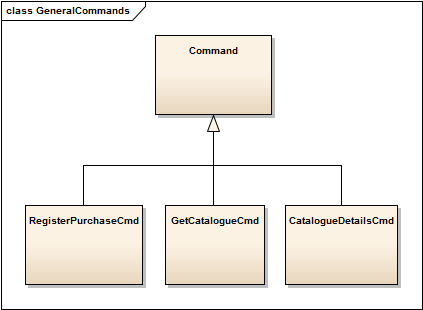
\includegraphics[width=0.6\textwidth]{Systemdesign/SharedLib/Images/Commands/GeneralCommands.png}
    \caption{Oversigt over generelle kommandoer der nedarver fra Command klassen}
    \label{fig:overklasseGen}
\end{figure}

\textbf{Produkt kommandoer} er kommando klasser der er specifikke for Product klassen og medfører ændringer i et givet produkt. Et eksempel på dette kunne være CreateProductCmd, som beder om et produkt skal oprettes i databasen.

På figur \ref{fig:overklassePrd} ses en oversigt over de forskellige produkt kommandoer der nedarver fra Command klassen.

\begin{figure}[H]
    \centering
    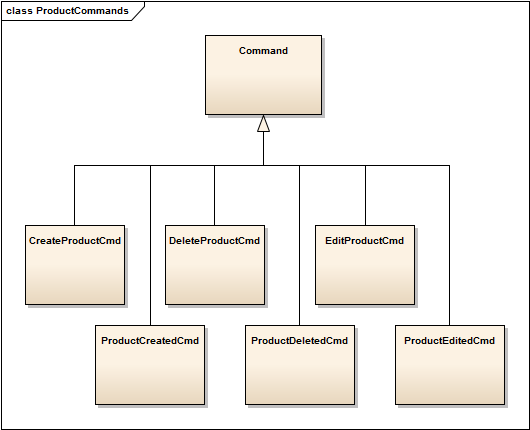
\includegraphics[width=0.6\textwidth]{Systemdesign/SharedLib/Images/Commands/ProductCommands.png}
    \caption{Oversigt over produktspecifikke kommandoer der nedarver fra Command klassen}
    \label{fig:overklassePrd}
\end{figure}

\textbf{Produktkategori kommadoer} er kommando klasser der er specifikke for ProductCategory klassen og disse medfører ændringer i den produktkategori der refereres. Et eksempel herpå kunne være DeleteProductCategoryCmd, der beder \gls{CS} om at slette den givne produktkategori fra databasen.

På figur \ref{fig:overklassePrdCat} ses en oversigt over de forskellige produktkategori kommandoer der nedarver fra Command klassen.

\begin{figure}[H]
    \centering
    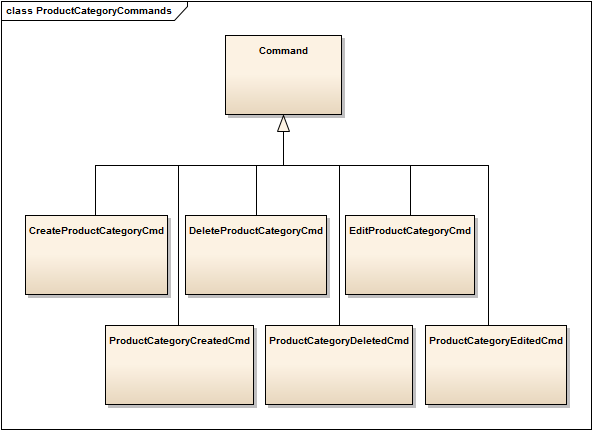
\includegraphics[width=0.6\textwidth]{Systemdesign/SharedLib/Images/Commands/ProductCategoryCommands.png}
    \caption{Oversigt over produktkategori-specifikke kommandoer der nedarver fra Command klassen}
    \label{fig:overklassePrdCat}
\end{figure}



\subsubsection{Klassebeskrivelser}
Herunder forklares yderligere om de forskellige kommando klasser der findes i \gls{SL}. Der vil desuden være en uddybende forklaring om de forskellige klassers funktionalitet og ansvar.\\

\textbf{Command}\\
Denne klasse indeholder blot en attribut, nemlig CmdName. Alle andre kommandoer i \gls{SL} nedarver fra denne klasse hvilket betyder at det bliver muligt at kode op imod en Command klasse og ved at caste på baggrund af CmdName, kan man generisk lave funktionalitet på modtagne kommando objekter, hvilket blandt andet bliver udnyttet i de forskellige marshallers Decode funktion.

\begin{figure}[H]
    \centering
    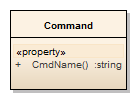
\includegraphics[width=0.2\textwidth]{Systemdesign/SharedLib/Images/Klasser/Command/Command.png}
    \caption{Command}
    \label{fig:klasseCMDCommand}
\end{figure}

\subsubsection*{Generelle kommandoer}

\textbf{RegisterPurchaseCmd}\\
Denne klasse indeholder en liste af købte produkter, PurchasedProduct objekter, og har til hensigt at sende en Purchase instans til \gls{CS} der her sørger for at gemme denne i databasen. Alt dette giver muligheden for at gemme tidligere salg, til senere evt. at kunne lave statistikker (fremtidigt arbejde) eller generere salgskviterringer og rekvisitionskvitteringer.

\begin{figure}[H]
    \centering
    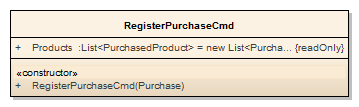
\includegraphics[width=0.6\textwidth]{Systemdesign/SharedLib/Images/Klasser/Command/RegisterPurchase.png}
    \caption{RegisterPurchaseCmd}
    \label{fig:klasseCMDRegP}
\end{figure}

\textbf{GetCatalogueCmd}\\
Denne klasse har intet indhold og dækker i virkeligheden kun et overfladisk behov for at kunne anmode om at få produktkataloget fra \gls{CS}. Derfor er Command klassens nedarvede attribut CmdName det eneste der er behov for i denne klasse.

\begin{figure}[H]
    \centering
    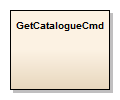
\includegraphics[width=0.2\textwidth]{Systemdesign/SharedLib/Images/Klasser/Command/GetCatalogue.png}
    \caption{GetCatalogueCmd}
    \label{fig:klasseCMDGetC}
\end{figure}

\textbf{CatalogueDetailsCmd}\\
Denne klasse er et modsvar til kommandoen GetCatalogue der anmoder om produktkataloget fra \gls{CS}, og vil derfor blive sendt som et modsvar med en liste af produktkategorier.

\begin{figure}[H]
    \centering
    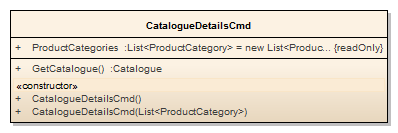
\includegraphics[width=0.6\textwidth]{Systemdesign/SharedLib/Images/Klasser/Command/CatalogueDetails.png}
    \caption{CatalogueDetailsCmd}
    \label{fig:klasseCMDGetC}
\end{figure}

\subsubsection*{Produkt kommandoer}

\textbf{CreateProductCmd/ProductCreatedCmd}\\
Disse klasser er skabt for henholdsvis at oprette et produkt i databasen og derefter en kommando der bliver sendt ud med information om at et nyt produkt er blevet oprettet. CreateProduct klassen indeholder alle de samme attributter som Product klassen med undtagelse af et produkt id da dette først er noget \gls{CS} tildeler produktet når det bliver oprettet i databasen. Derfor er der naturligvis en ekstra attribut i ProductCreated, der hedder ProductId, som er dette id der er blevet tildelt produktet, og som senere kan bruges som reference til dette produkt.

\begin{figure}[H]
    \centering
    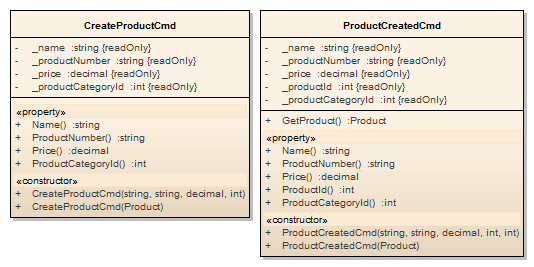
\includegraphics[width=0.8\textwidth]{Systemdesign/SharedLib/Images/Klasser/Command/Product/CreatePrd.png}
    \caption{CreateProductCmd/ProductCreatedCmd}
    \label{fig:klasseCMDCreatePrd}
\end{figure}

\textbf{DeleteProductCmd/ProductDeletedCmd}\\
DeleteProduct og ProductDeleted er to klasser med praktisk talt samme informationer. Den springende forskel er blot at DeleteProduct bliver sendt til \gls{CS} for at bede denne om at slette produktet fra databasen, og ProductDeleted er et svar fra \gls{CS} ud til alle interessanter om at det omtalte produkt er blevet slettet fra databasen.
Klasserne indeholder naturligvis samme attributter som Product klassen da disse informationer kan være relevante for de forskellige modtagere. For at anmode om sletning af et produkt kan man dog blot nøjes med at sende produkt id'et med kommandoen og ud fra dette kan \gls{CS} finde produktet i databasen og slette det.

\begin{figure}[H]
    \centering
    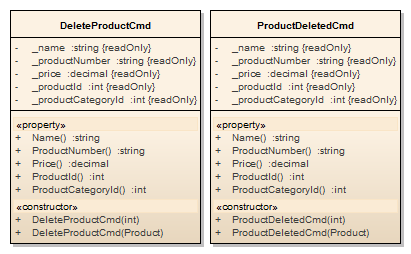
\includegraphics[width=0.6\textwidth]{Systemdesign/SharedLib/Images/Klasser/Command/Product/DeletePrd.png}
    \caption{DeleteProductCmd/ProductDeletedCmd}
    \label{fig:klasseCMDDeletePrd}
\end{figure}

\textbf{EditProductCmd/ProductEditedCmd}\\
Disse klasser bruges af de forskellige systemer til at lave ændringer i et allerede eksisterende produkt, f.eks. hvis et produkts name attribute er stavet forkert, så kan der sendes et EditProduct objekt med de reviderede informationer til \gls{CS} og denne vil herefter sørge for at rette disse informationer i databasen. ProductEdited kommandoen er herefter de opdaterede informationer der bliver sendt ud til alle interessanter i systemet. De to klasser indeholder derfor også alle de samme informationer som Product klassen og der kan på den måde også ændres flere informationer på et produkt i samme kommando.

\begin{figure}[H]
    \centering
    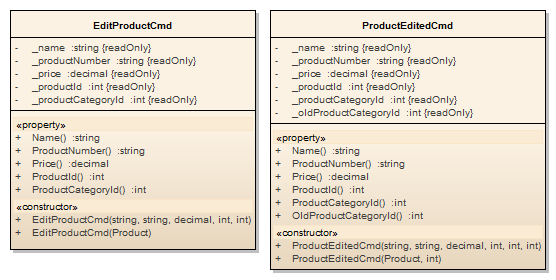
\includegraphics[width=0.8\textwidth]{Systemdesign/SharedLib/Images/Klasser/Command/Product/EditPrd.png}
    \caption{EditProductCmd/ProductEditedCmd}
    \label{fig:klasseCMDDeletePrd}
\end{figure}

\subsubsection*{Produktkategori kommandoer}

\textbf{CreateProductCategoryCmd/ProductCategoryCreatedCmd}\\
Disse klasser er skabt for at oprette en produktkategori i databasen, CreateProductCategory anmoder \gls{CS} om dette og derefter sender denne en ProductCategoryCreated kommando ud med information om at en ny produktkategori er blevet oprettet. CreateProductCategory klassen indeholder alle de samme attributter som ProductCategory klassen med undtagelse af et produktkategori id da dette først er noget \gls{CS} tildeler produktkategorien når denne bliver oprettet i databasen. Derfor er der naturligvis en ekstra attribut i ProductCategoryCreated, der hedder ProductCategoryId, som er det id der er blevet tildelt produktkategorien, og som senere kan bruges som reference til denne produktkategori. 

\begin{figure}[H]
    \centering
    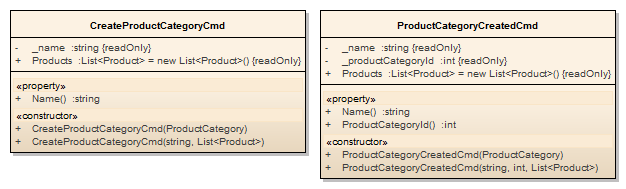
\includegraphics[width=1.0\textwidth]{Systemdesign/SharedLib/Images/Klasser/Command/ProductCategory/CreatePrdCtg.png}
    \caption{CreateProductCategoryCmd/ProductCategoryCreatedCmd}
    \label{fig:klasseCMDCreatePrdCtg}
\end{figure}

\textbf{DeleteProductCategoryCmd/ProductCategoryDeletedCmd}\\
DeleteProductCategory og ProductCategoryDeleted er to klasser med praktisk talt samme informationer. Den springende forskel er blot at DeleteProductCategory bliver sendt til \gls{CS} for at bede denne om at slette produkkategorien fra databasen, og ProductCategoryDeleted er et svar fra \gls{CS} ud til alle interessanter om at den omtalte produktkategori er blevet slettet fra databasen.
Klasserne indeholder naturligvis samme attributter som ProductCategory klassen da disse informationer kan være relevante for de forskellige modtagere. For at anmode om sletning af en produktkategori kan man dog blot nøjes med at sende produktkategori id'et med kommandoen og ud fra dette kan \gls{CS} finde produktkategorien i databasen og slette den.


\begin{figure}[H]
    \centering
    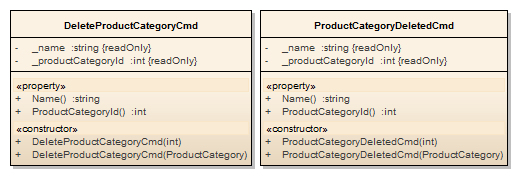
\includegraphics[width=0.8\textwidth]{Systemdesign/SharedLib/Images/Klasser/Command/ProductCategory/DeletePrdCtg.png}
    \caption{DeleteProductCategoryCmd/ProductCategoryDeletedCmd}
    \label{fig:klasseCMDDeletePrdCtg}
\end{figure}

\textbf{EditProductCategoryCmd/ProductCategoryEditedCmd}\\
Disse klasser bruges af de forskellige systemer til at lave ændringer i et allerede eksisterende produktkategorier, f.eks. hvis en produktkateogri's name attribute er stavet forkert, så kan der sendes et EditProductCategory objekt med de reviderede informationer til \gls{CS} og denne vil herefter sørge for at rette disse informationer i databasen. ProductCategoryEdited kommandoen er herefter de opdaterede informationer der bliver sendt ud til alle interessanter i systemet. De to klasser indeholder derfor også alle de samme informationer som ProductCategory klassen og der kan på den måde også ændres flere informationer på et produktkategori i samme kommando.


\begin{figure}[H]
    \centering
    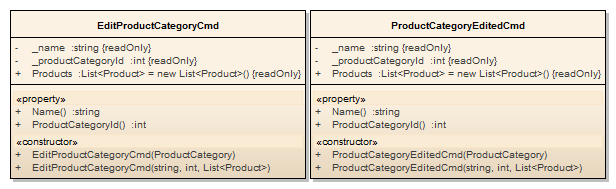
\includegraphics[width=1.0\textwidth]{Systemdesign/SharedLib/Images/Klasser/Command/ProductCategory/EditPrdCtg.png}
    \caption{EditProductCategoryCmd/ProductCategoryEditedCmd}
    \label{fig:klasseCMDEditPrdCtg}
\end{figure}



